\documentclass[11pt]{article}
\usepackage[paper=letterpaper, left=1in, right=1in, top=1in, bottom=1in]
           {geometry}
\usepackage[parfill]{parskip}
\usepackage{amsmath}
\usepackage{graphicx}
\usepackage{fancyvrb}
\usepackage{upquote}
\usepackage[en-GB]{datetime2}
\DTMlangsetup[en-GB]{ord=omit}
\usepackage{xfrac}

\newcommand{\problem}[1]{\textbf{Problem #1 ---} }
\newcommand{\answer}{\textit{Answer: } }

\begin{document}
\thispagestyle{empty}

\begin{center}
{\large CS 310}\\
Assignment 0904
\end{center}

\begin{flushright}
Bill Jin
\end{flushright}

\problem{1} Use the definitions to prove or disprove the statement
$2n^2 + 3 \in O(n^3)$, and illustrate this graphically.

\answer The definition requires us to find $c$ and $n_0$ so that
$2n^2 + 3 \leq cn^3$ when $n \geq n_0$.\\
Based on the definition n and c are both non-negative constants. Since we have:

\[2n^2 + 3 \leq cn^3\]

\[ \frac{2n^2 + 3}{n^3} \leq c\]
And raise the degree of all other terms as the highest one including constants with n.
\[ \frac{2n^2 + 3}{n^3} \leq \frac{2n^3 + 3n^3}{n^3} \text{ (for all $n_0 \geq$ 1)}\]
Obviously, the right-hand will be definitely higher or equal to the left-side for all $n_0 \geq$ 1.
Then, cancel all the terms and end with a constant:
\[\frac{2n^2 + 3}{n^3} \leq 5 \text{ (for all $n_0 \geq$ 1)}\]

\[c = 5 \text{ (for all $n_0 \geq$ 1)}\]

Therefore, we conclude that $2n^2 + 3 \in O(n^3)$ is true since we have $2n^2 + 3 \leq 5n^3$.


This is graphically illustrated by the following plot that shows
$2n^2 + 3$ along with the standard function $n^3$ scaled by
the constant coefficient $c = 5$, for all n $\geq$ 1.

\begin{figure}[htbp]
\centerline{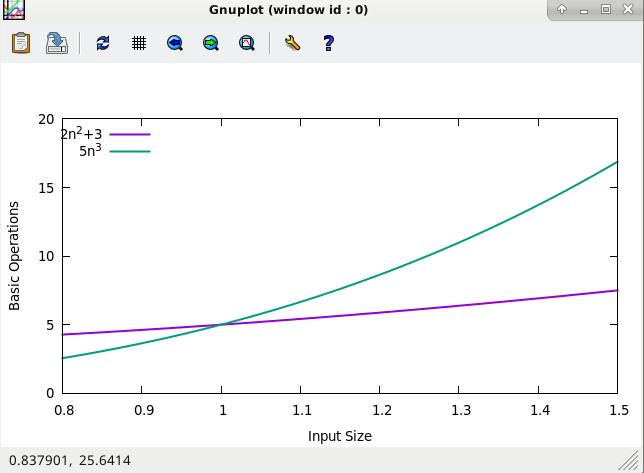
\includegraphics[scale = 0.3]{problem_1.png}}
\caption{The graph shows y = $2n^2$ + 3 and y = $5n^3$}
\label{fig}
\end{figure}

% change 0.7 below depending on the size of your image
% make sure the image fits on the page and is legible, without
% noticeable pixellation
%\begin{center}
%  \includegraphics[width=0.7\textwidth]{problem1.png}
%\end{center} 

\problem{2} Either prove the following assertion using the definitions
or disprove it with a specific counterexample:
\[\text{if } T(n) \in O(S(n)) \text{ then } S(n) \in \Omega(T(n))\]

\answer If T(n) $\in$ O(S(n)), then there is a constant c which is great and equal to zero 
(c $\geq$ 0), and a constant $n_0$ which that n is great or equal to $n_0$(n $\geq$ $n_0$), where we can conclude:
\[\text{T(n)} \leq c \times S(n)\]

We can divide both sides of the expression by the constant c, then we have:
\[\frac{1}{c} \times T(n) \leq S(n) \text{ (for $\frac{1}{c}$ $>$ 0 and n $\geq$ $n_0$.)}\]


Therefore, there is a constant $\frac{1}{c}$. which can be replaced by constant k. Then we can conclude:
\[
S(n) \geq k \times T(n)
\]
for k $>$ 0 and n $\geq$ $n_0$, which is exact definition of S(n) $\in \Omega$ (T(n)).

\problem{3} For the following algorithm, explain what it computes,
state what the input size for analysis is, state what basic operations
should be counted for analyzing it, state exactly how many operations
are executed as a function of the input size, and state the efficiency
class to which it belongs.

\begin{Verbatim}[numbers=left,xleftmargin=5mm]
void foo(vector<unsigned>& array)
{
  size_t n = array.size();
  for (size_t pass_indx = 0; pass_indx < n - 1; pass_indx++)
  {
    size_t min_position = pass_indx;
    for (size_t compare_indx = pass_indx + 1; compare_indx < n; 
         compare_indx++)
    {
      if (array.at(compare_indx) < array.at(min_position))
      {
        min_position = compare_indx;
      }
    }

    if (min_position != pass_indx)
    {
      swap(array.at(pass_indx), array.at(min_position));
    }
  }
}
\end{Verbatim}

\answer This algorithm is used to sort the elements in the vector from minimum to maximum.
Consider line 3, which defines \texttt{n}. This allows us to see
that the input size is the size of the vector. 

For the worst cases (Big-O), the operations that are counted are:
\begin{itemize}
\item the assignment on line 3, we count as 1 operation, 
\item the for loop condition on line 4, we count as 2n operations,
\item the \texttt{min\_position} assignment on line 5, we count as (n-1) operations,
\item the second for loop condition on line 7 and 8 will are counted as (n)+(n-1)+(n-2)..+2 number of times, which is $\frac{(n+2)(n-1)}{2}$, and have two operations each time, so we count (n+2)(n-1) number of operation,
\item the if condition on line which is comparison on line 10, we count as (n-1)+(n-2)+...1, which is $\frac{n^2-n}{2}$,
\item the assignment of \texttt{min\_position} inside the if statement on line 12, we count as (n-1)+(n-2)+...1, which is also $\frac{n^2-n}{2}$,
\item the \texttt{min\_position} comparison in if condition on line 16, we count as (n-1) operations,
\item and the swap function on line 18, we count as 2(n-1),
\end{itemize}

After sum up all, the number of times of all operations that are executed is:
\[
2n^2+6n-5
\]

For the best cases (Big-$\Omega$), the operations that are counted are:
\begin{itemize}
\item the assignment on line 3, we count as 1 operation, 
\item the for loop condition on line 4, we count as 2n operations,
\item the \texttt{min\_position} assignment on line 5, we count as (n-1) operations,
\item the second for loop condition on line 7 and 8 will are counted as (n)+(n-1)+(n-2)..+2 number of times, which is $\frac{(n+2)(n-1)}{2}$, and have two operations each time, so we count (n+2)(n-1) number of operation
\item the if condition on line which is comparison on line 10, we count as (n-1)+(n-2)
+...1, which is $\frac{n^2-n}{2}$,
\item the assignment of \texttt{min\_position} inside the if statement on line 12, we count as 0 based on best case.
\item the \texttt{min\_position} comparison in if condition on line 16, we count as (n-1) operations,
\item and the swap function on line 18, we count as 0 times, since this is best case.
\end{itemize}

After sum up all, the number of times of all operations that are executed is:
\[
n^2+5n+\frac{n^2-n}{2}-1
\]

Since there are two if conditions which could cause the best and the worst cases. Therefore, we can find out that this algorithm belongs to Big-Oh and Big-Omega efficiency class.

\[
    T(n) \in O(n^2) \text{ for c = 4, all n $\geq$ 0}    
\]
\[
    T(n) \in \Omega(n^2) \text{ for c = 1, all n $\geq$ 0}    
\]

or equivalently,

\[
T(n) \in \Theta(n^2)
\]

\problem{4} Write a C++ program that implements the algorithm
in problem 3, counts the number of basic operations, and outputs the
input size and the count of basic operations to the cerr stream. 

\answer See the submitted file HM.cpp

\problem{5} Run your program from problem 4 many times with many
different inputs and capture the results.  Using the output of the,
create a plot of input size vs.\ basic operations, along with one or
more standard functions properly scaled, to illustrate the analysis
you obtained in Problem 3.

\answer When the program is run with the command

\begin{Verbatim}
for n in `seq 10 10 1000`
do
    ./program $n > /dev/null
    ./program $n > /dev/null
done 2> results.dat
\end{Verbatim}

and the resulting data file is plotted, we get the following. Also
plotted on the same axes are the scaled standard functions $3n^2$ and
$n^2$ which illustrate that the algorithm is big-theta.

\begin{center}
  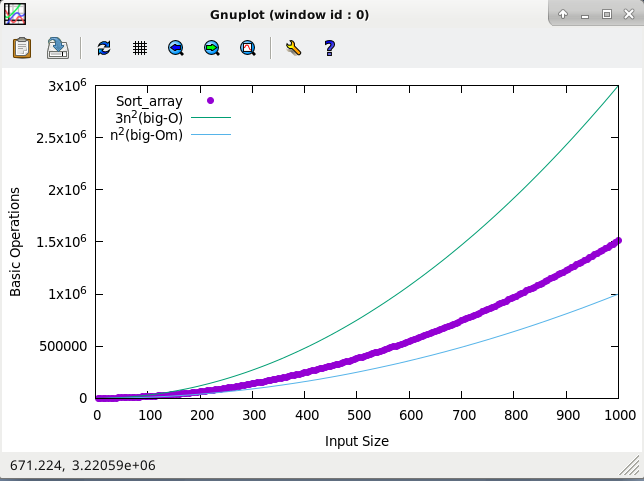
\includegraphics[width=0.7\textwidth]{problem_5.png}
\end{center} 

\end{document}


